\chapter{Additional Configurations} \label{ch: additional configurations}

To draw a full picture, plenty of approaches which had the goal to improve the results will be mentioned in this chapter. Sadly, no one changed the outcome by any means. Facing this was an enormous obstacle while researching. Some of them will be presented shortly in this chapter. In all cases, it is obvious that these configurations were dead ends.

% --------------------------------------
\clearpage
\section{Multiple hidden layers} \label{subsubsec: multiple hidden layers}
Different numbers of layers ranging from $ 1 $ to $ 100 $ were tested, some example results will be depicted.
\newcommand{\hh}{0.365\textheight}
%
\begin{figure}[H]
	\centering
	\subcaptionbox{\gls{sr} of a model using English and \onehot{s} with $ 40 $ hidden layers.}{
		
\includegraphics[height=\hh]{Bilder/chapter4/additional_configurations/OHE_OHE_4000E_100BS_40L_1C_200P_1500T_J/Transition_Probability_Matrix;_t=1,_DF=0.5.png}
	}
	\hfill
	\subcaptionbox{\gls{mds} of the matrix in (a).}{
		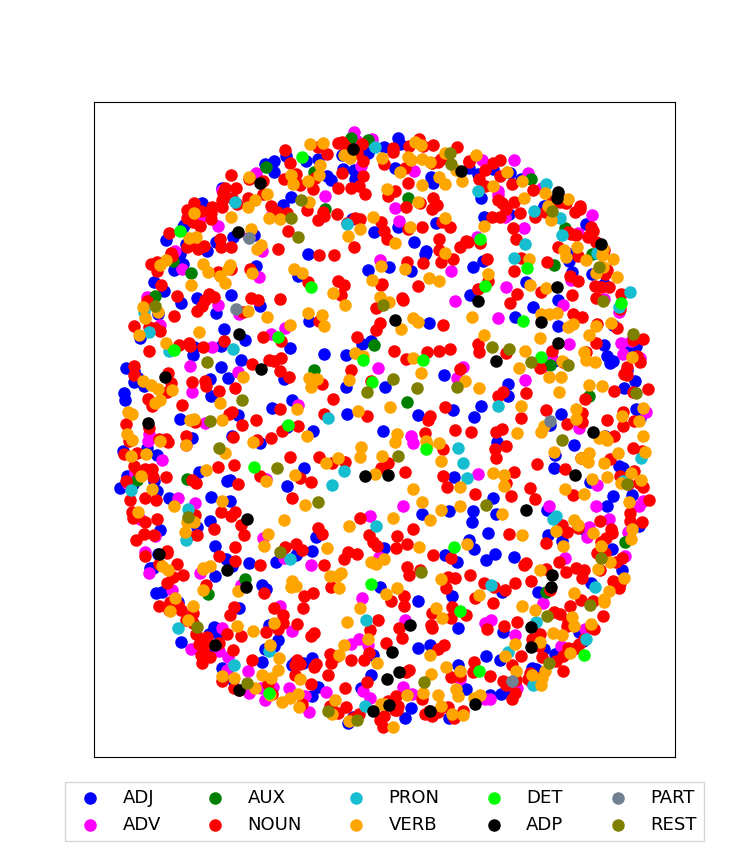
\includegraphics[height=\hh]{Bilder/chapter4/additional_configurations/OHE_OHE_4000E_100BS_40L_1C_200P_1500T_J/MDS_of_Transition_Probability_Matrix;_t=1,_DF=0.5.png}
	}
	\caption{Although mentioned that transition probability matrices don't show anything if too many words are used, they can be used sometimes to detect failure. The reference, at least for the \gls{mds}, is illustrated in \figref{\ref{fig: w2w model gt en}}. The value of the metric is $ 0.50 $, the equivalent with one layer achieves $ 0.10 $. This could imply that more layers hamper learning.}
	\label{fig: text model en ohe 40L}
\end{figure}
%
\clearpage
\begin{figure}[H]
	\centering
		\subcaptionbox{\gls{sr} of a model using English and \onehot{s} with $ 10 $ hidden layers.}{
			
\includegraphics[height=\hh]{Bilder/chapter4/additional_configurations/OHE_OHE_7000E_100BS_10L_1C_200P_1500T_J/Transition_Probability_Matrix;_t=1,_DF=0.5.png}
		}
%	\subcaptionbox{\gls{mds} of a model using english and \onehot{s} with $ 2 $ hidden layers.}{
%		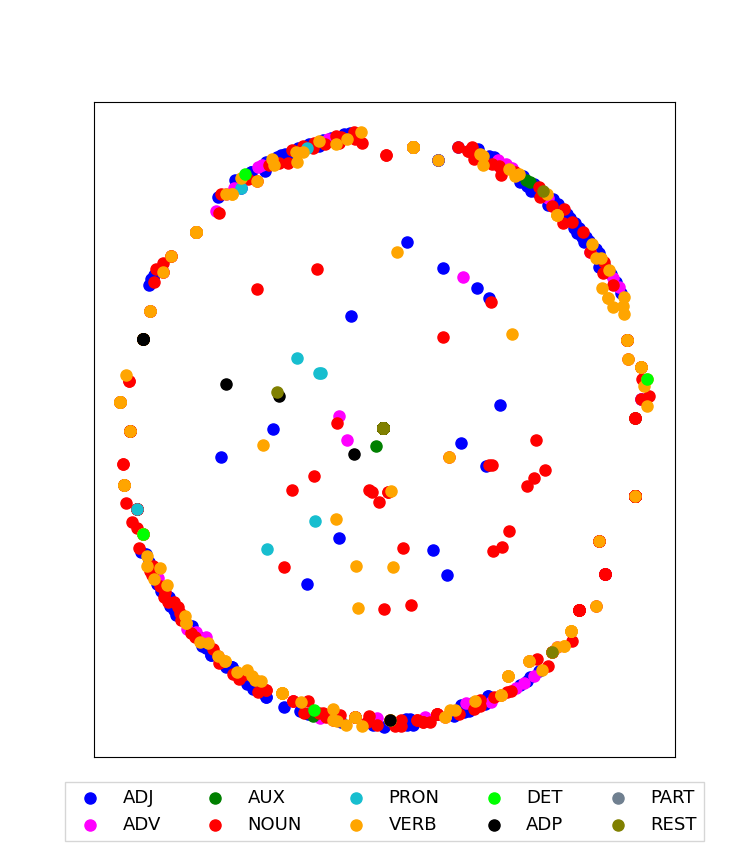
\includegraphics[height=\hh]{Bilder/chapter4/additional_configurations/OHE_OHE_4000E_100BS_2L_1C_200P_1500T_J/MDS_of_Transition_Probability_Matrix;_t=1,_DF=0.5.png}
%	}
	\hfill
	\subcaptionbox{\gls{mds} of a model using English and \onehot{s} with $ 2 $ hidden layers.}{
		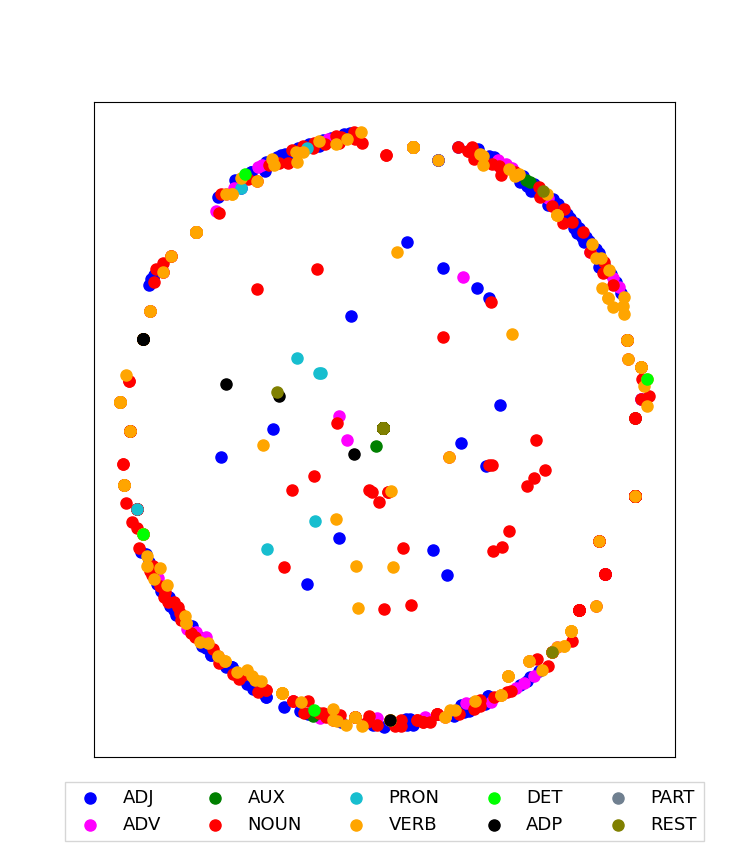
\includegraphics[height=\hh]{Bilder/chapter4/additional_configurations/OHE_OHE_4000E_100BS_2L_1C_200P_1500T_J/MDS_of_Transition_Probability_Matrix;_t=1,_DF=0.5.png}
	}
%	\subcaptionbox{\gls{sr} of a model using english and \onehot{s} with $ 10 $ hidden layers.}{
%		
\includegraphics[height=\hh]{Bilder/chapter4/additional_configurations/OHE_OHE_7000E_100BS_10L_1C_200P_1500T_J/Transition_Probability_Matrix;_t=1,_DF=0.5.png}
%	}
	\caption{As mentioned before, more layers result in a worse \gls{sr}. Already one additional hidden layer lowers the metric. The model in (a) reaches $ 0.22 $, whereas with one hidden layer the value is $ 0.10 $. The network in (b) was configured with $ 2 $ hidden layers and the successor representation looks indistinguishable from one training with $ 40 $ (\figref{\ref{fig: text model en ohe 40L}}).}
\end{figure}

% --------------------------------------

\clearpage
\section{Many epochs and multiple hidden layers}
The example outputs stem from a model which was trained with sixfold epochs and $ 40 $ hidden layers.
\begin{figure}[H]
	\centering
		\subcaptionbox{\gls{sr} of a model using English, \onehot{s}, $ 25,000 $ epochs and $ 40 $ layers.}{
		
\includegraphics[height=\twocolpicheight]{Bilder/chapter4/additional_configurations/OHE_OHE_25000E_100BS_40L_1C_200P_1500T_J/Transition_Probability_Matrix;_t=1,_DF=0.5.png}
	}
	\hfill
	\subcaptionbox{\gls{mds} of a model using English, word vectors, $ 25,000 $ epochs and $ 40 $ layers}{
		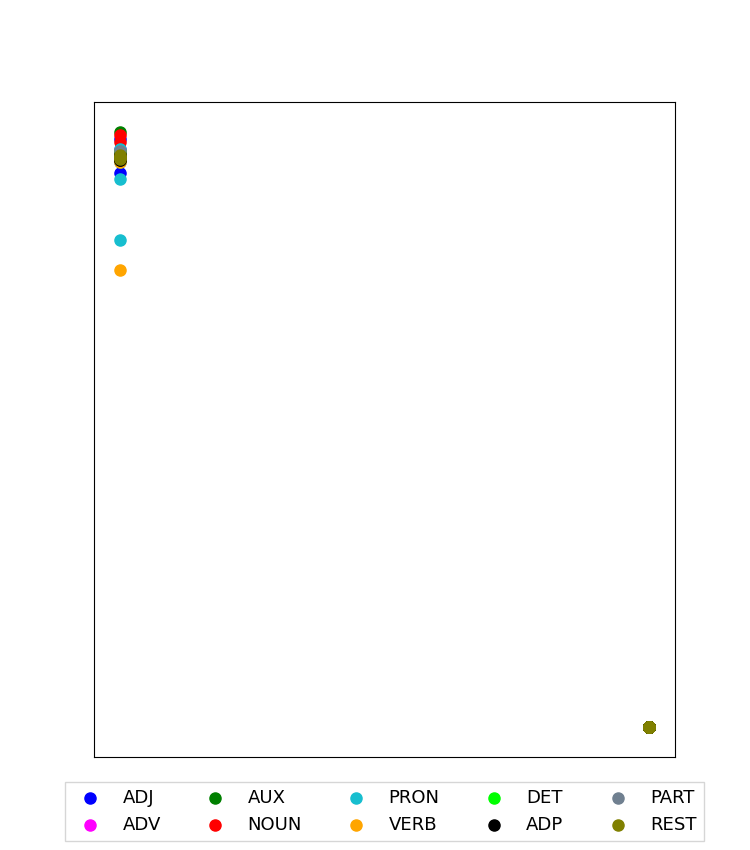
\includegraphics[height=\twocolpicheight]{Bilder/chapter4/additional_configurations/W2V_W2V_25000E_100BS_40L_1C_200P_1500T_J/MDS_of_Transition_Probability_Matrix;_t=1,_DF=0.5.png}
	}
%	\caption{The only conclusion to draw from this plot of two different models is that additional epochs might lead to a full degeneration of the results if word vectors are used for training. The \onehot{} analogue shows no mismatch to them of \secreff{subsubsec: multiple hidden layers}.}
	\caption{Trying a combination of numerous epochs in combination with a relative high number of hidden layers leaves a degenerated result.}
\end{figure}

% --------------------------------------

\clearpage
\section{Using word vectors to learn a \onehot{}}
This configuration is a combination of the two mainly used in the thesis. It uses word vectors as input and \onehot{s} as output \ie heterogeneous structured training data.
\begin{figure}[H]
	\centering
	\subcaptionbox{English, word vector to \onehot{} as \gls{mds}.}{
		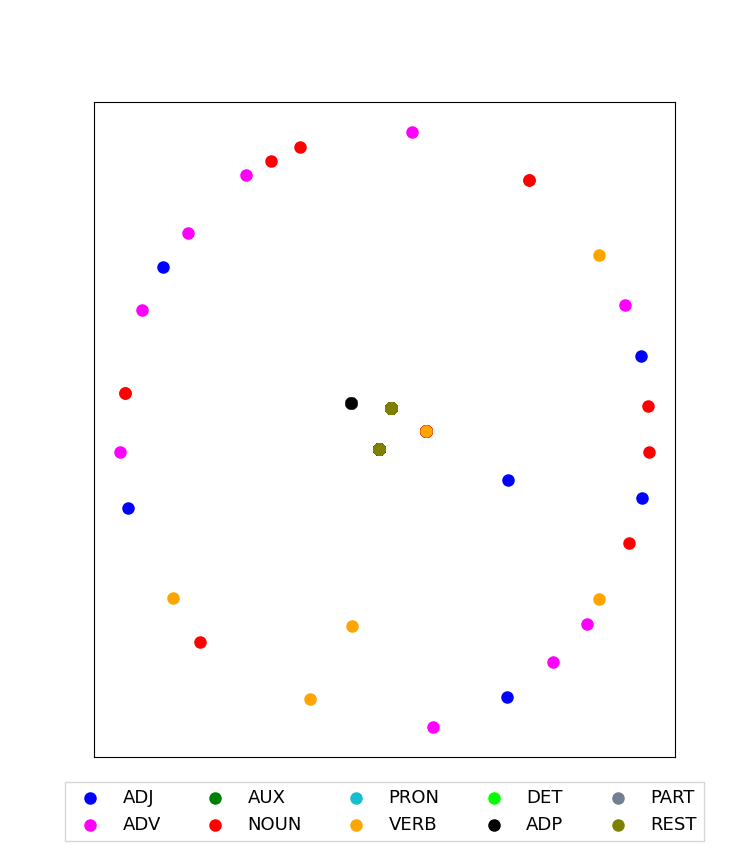
\includegraphics[width=\twocolpicwidth]{Bilder/chapter4/additional_configurations/W2V_OHE_5000E_100BS_1L_1C_200P_1500T_D/MDS_of_Transition_Probability_Matrix;_t=1,_DF=0.5.png}
	}
	\hfill
	\subcaptionbox{German, ground truth \gls{mds} of word to word transitions.}{
		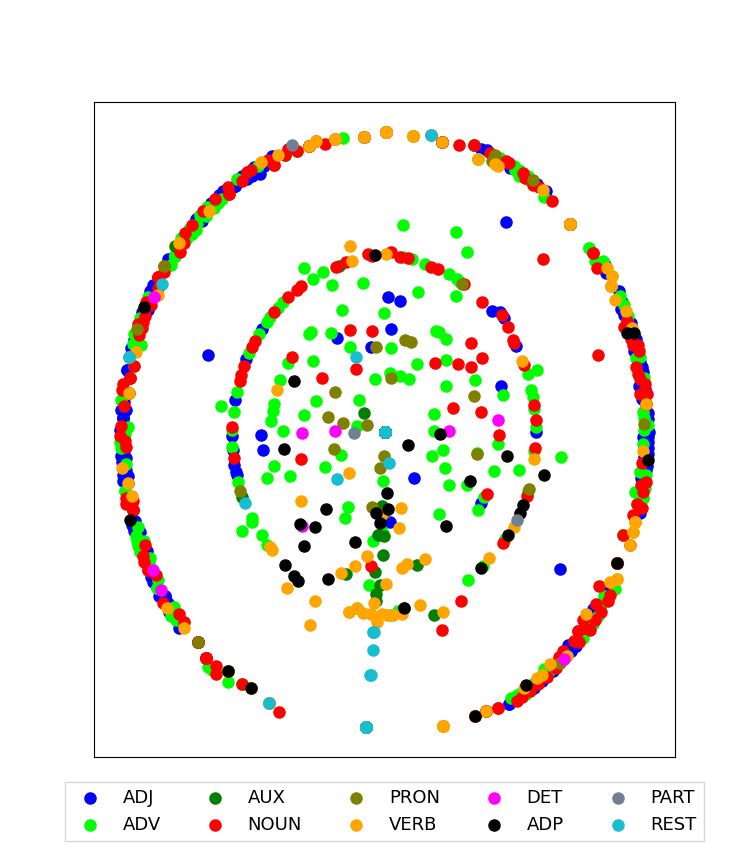
\includegraphics[width=\twocolpicwidth]{Bilder/chapter4/W2W/ground_truths/MDS_D_200pages_1500T_words.png}
	}
	\caption{\gls{mds} plot of a model using german training data and word vectors as input to learn an \onehot{}. The results lack characteristics to draw sensible conclusions from. Though, it is possible to calculate the metric for the configuration: $ 0.47 $. By comparing it with \tabref{\ref{tab: text model versions and metrics}}, it is situated between its full \onehot{} and word vector relatives.}
\end{figure}

% --------------------------------------

\clearpage
\section{Multiplying the training data} \label{subsubsec: multiplying training data}
The goal of multiplying the training data \ie concatenating the training data $ n $ times with itself, was to have the opportunity to process the training data more often during one epoch.
\begin{figure}[H]
	\centering
	\subcaptionbox{German, \onehot{s} with $ 5 $ concatenations.}{
		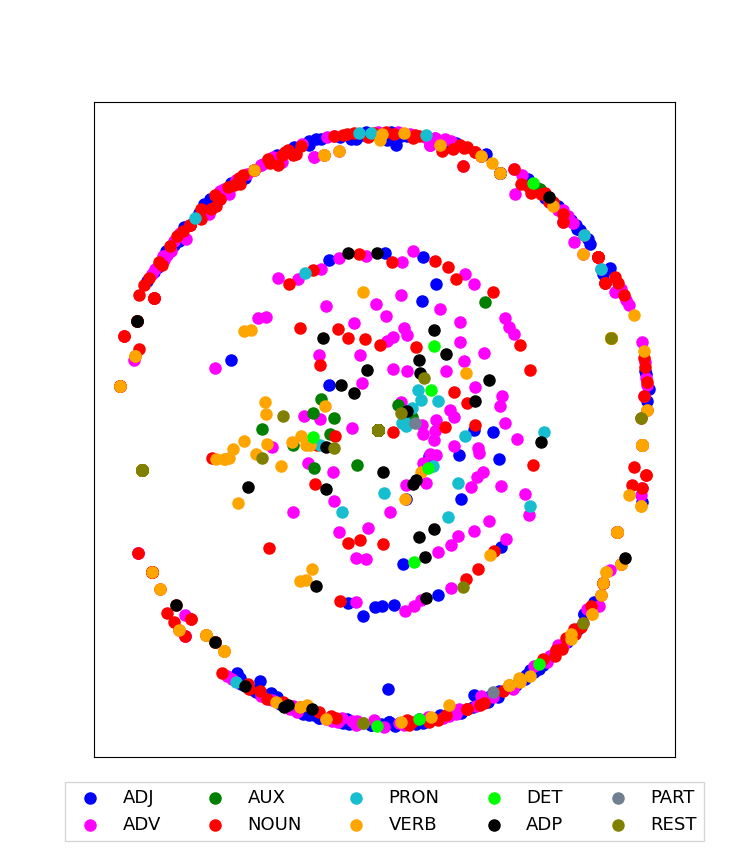
\includegraphics[width=\twocolpicwidth]{Bilder/chapter4/additional_configurations/OHE_OHE_5000E_100BS_1L_5C_200P_1500T_D/MDS_of_Transition_Probability_Matrix;_t=1,_DF=0.5.png}
	}
	\hfill
	\subcaptionbox{German, word vectors with $ 5 $ concatenations.}{
		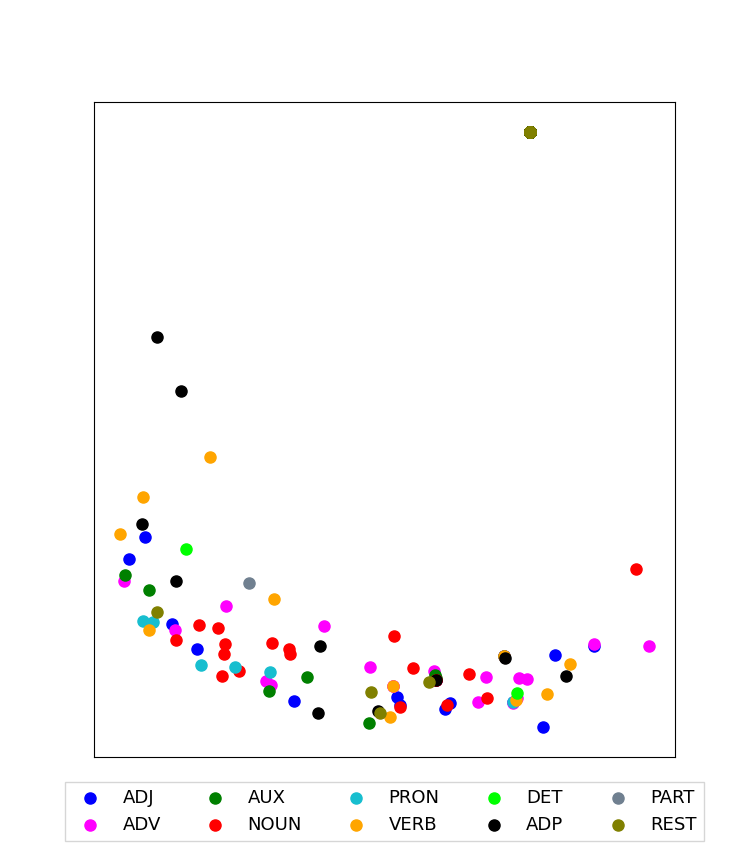
\includegraphics[width=\twocolpicwidth]{Bilder/chapter4/additional_configurations/W2V_W2V_5000E_100BS_1L_5C_200P_1500T_D/MDS_of_Transition_Probability_Matrix;_t=1,_DF=0.5.png}
	}
	\caption{Concatenating the training data $ 5 $ times with itself doesn't change outcomes (compare \figref{\ref{fig: text model cumulativ mds plots}}). This impression is fortified by the metrics both models achieve: $ 0.14 $ for \onehot{s} and $ 0.72 $ with word vectors ($ 0.08 $ and $ 0.74 $ without respectively, \tabref{\ref{tab: text model versions and metrics}}).}
\end{figure}

% --------------------------------------

\clearpage
\section{Calculating high time steps}
One idea was to calculate high time steps of the \gls{sr} hoping the irregularities even out in distant future.
\begin{figure}[H]
	\centering
	\subcaptionbox{\gls{mds} of a \gls{sr} with $ t = 20 $. German and \onehot{s} were used during training.}{
		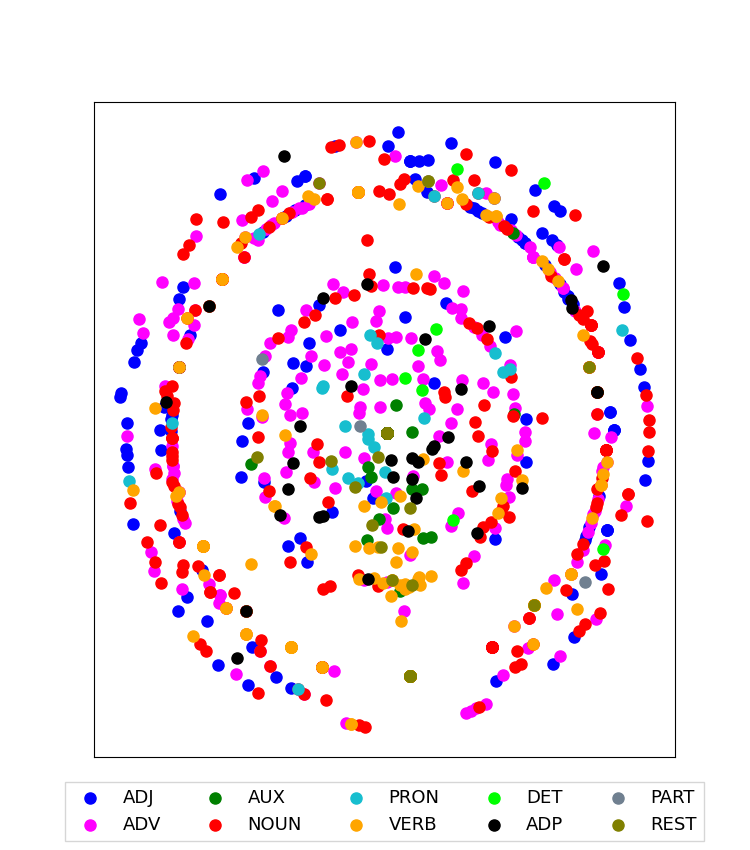
\includegraphics[width=\twocolpicwidth]{Bilder/chapter4/additional_configurations/hohes_t/OHE_OHE_5000E_100BS_1L_1C_200P_1500T_D/MDS_of_SR,_t=20,_DF=0.5.png}
	}
	\hfill
	\subcaptionbox{\gls{mds} of a \gls{sr} with $ t = 50 $. German and \onehot{s} were used during training.}{
		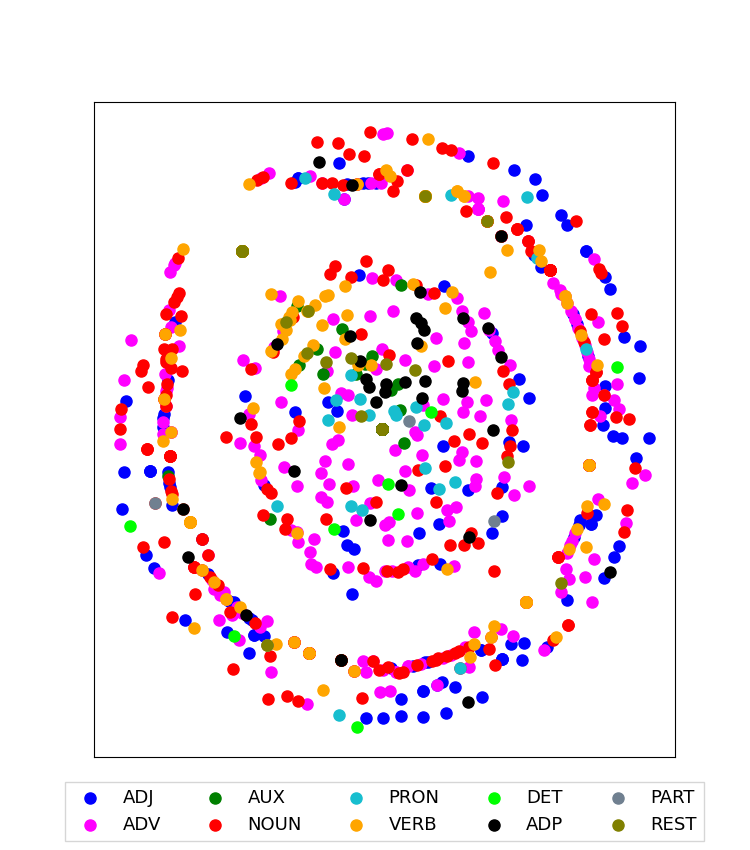
\includegraphics[width=\twocolpicwidth]{Bilder/chapter4/additional_configurations/hohes_t/OHE_OHE_5000E_100BS_1L_1C_200P_1500T_D/MDS_of_SR,_t=50,_DF=0.5.png}
	}
	\caption{High time steps also don't facilitate progress since no evident structure is recognizable within the plots. A comparison with the ground truth wouldn't add additional insights too because the underlying matrices can't be interpreted as transition probability matrices.}
	\label{fig: high time steps ohe}
\end{figure}
%
\clearpage
\begin{figure}[t]
	\centering
	\subcaptionbox{\gls{mds} of a \gls{sr} with $ t = 20 $. German and word vectors were used during training.}{
		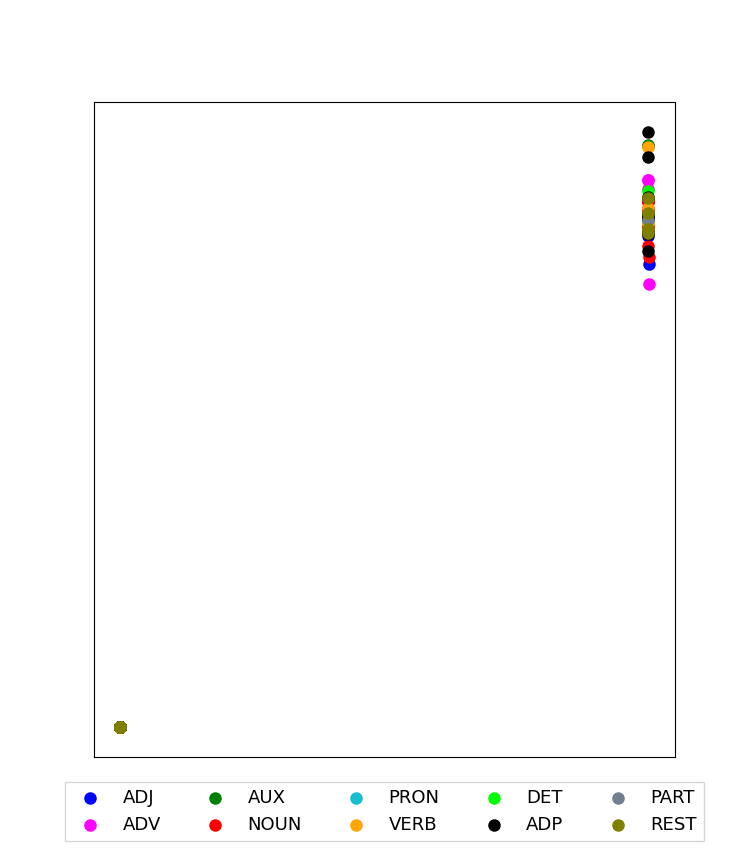
\includegraphics[width=\twocolpicwidth]{Bilder/chapter4/additional_configurations/hohes_t/W2V_W2V_5000E_100BS_1L_1C_200P_1500T_D/MDS_of_SR,_t=20,_DF=0.5.png}
	}
	\hfill
	\subcaptionbox{\gls{mds} of a \gls{sr} with $ t = 50 $. German and word vectors were used during training.}{
		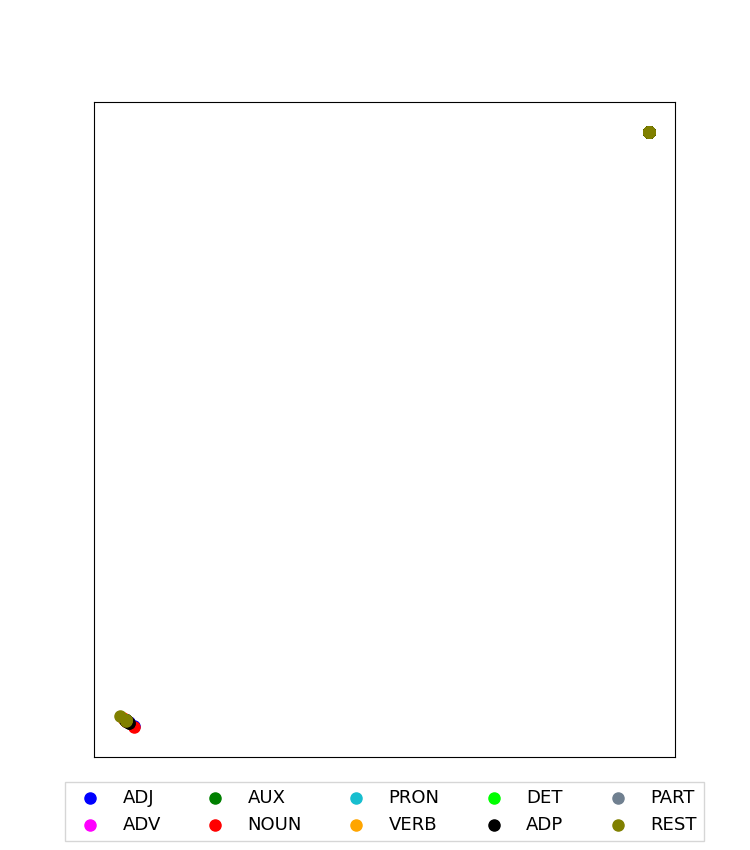
\includegraphics[width=\twocolpicwidth]{Bilder/chapter4/additional_configurations/hohes_t/W2V_W2V_5000E_100BS_1L_1C_200P_1500T_D/MDS_of_SR,_t=50,_DF=0.5.png}
	}
	\caption{As before in \figref{\ref{fig: high time steps ohe}} no structure is recognizable to do further research on. Results relying on word vectors again seem to be very labile and one dimensional.}
\end{figure}

% --------------------------------------

\clearpage
\section{Predict only the most frequent words}
Similar to \secreff{subsubsec: multiplying training data}, the most frequent words of the text are seen more often by the network. Hence, it might be able to learn these inputs better than ordinary ones.
\begin{figure}[H]
	\centering
	\subcaptionbox{German with word vectors. \gls{mds} of the $ 40 $ most frequent words.}{
		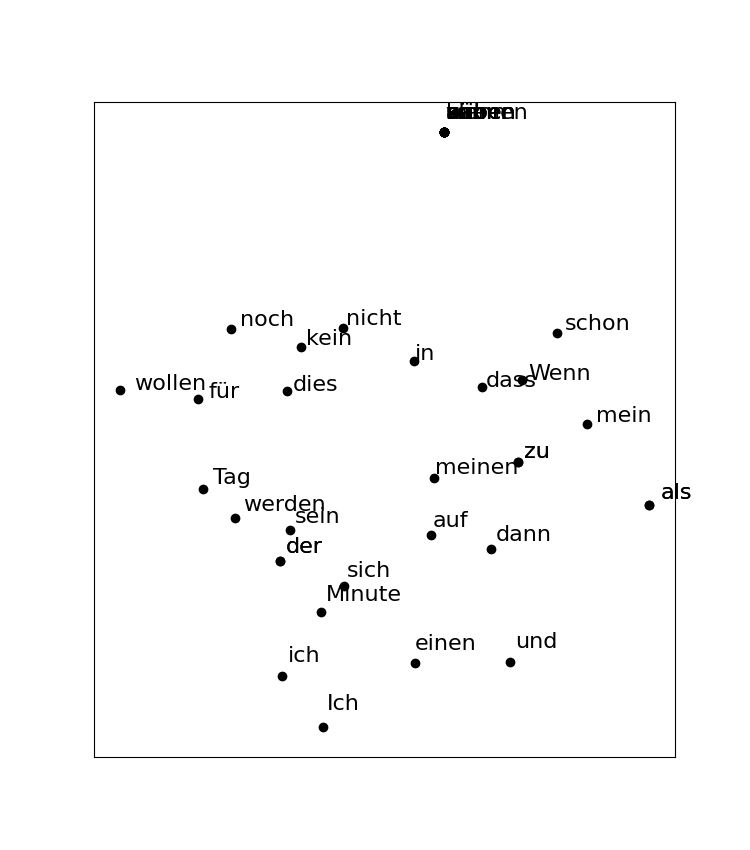
\includegraphics[width=\twocolpicwidth]{Bilder/chapter4/additional_configurations/MostFrequentWords_4000E_100BS_1L_1C_200P_1500T_D/MDS_of_Transition_Probability_Matrix;_t=1,_DF=0.5.png}
	}
	\hfill
	\subcaptionbox{Same \gls{mds} plot as in (a) but annotated with \postag{s} instead of words.}{
		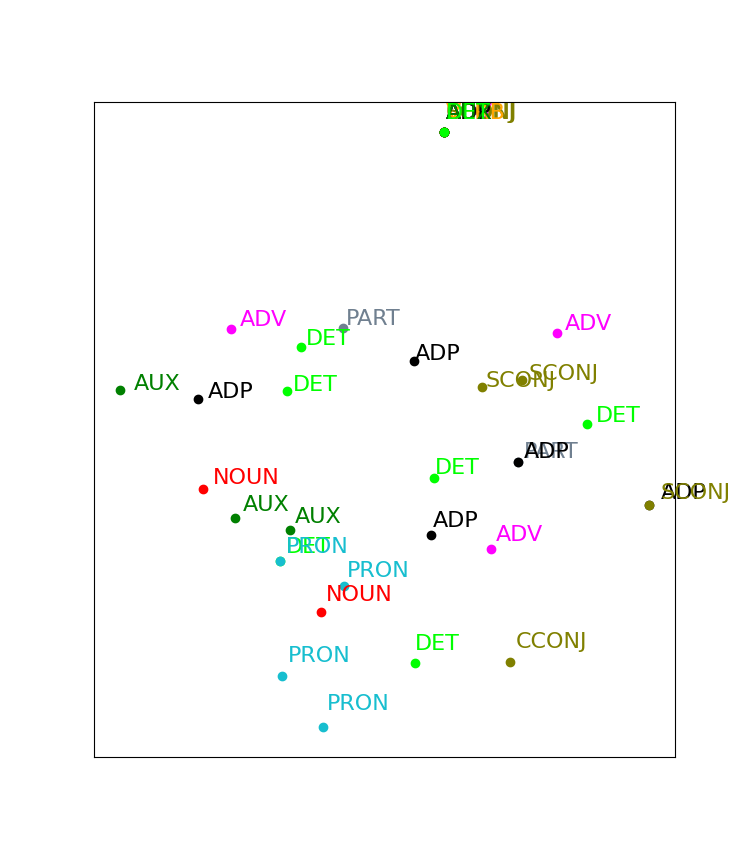
\includegraphics[width=\twocolpicwidth]{Bilder/chapter4/additional_configurations/MostFrequentWords_4000E_100BS_1L_1C_200P_1500T_D/ud_pos_tag_annotated.png}
	}
	\caption{The same model with a german data set and word vectors as in \secreff{sec: text based models and architecture} was trained. Predictions were limited to the $ 40 $ most frequent words. For a better overview the second plot was labeled with the corresponding \postag{s}.}
\end{figure}
